\section{Modellierung}


\subsection{Einheiten}
Die Basiseinheit ist Milimeter. Es ist jedoch möglich mit anderen SI-Einheiten (m, dm oder cm) zu arbeiten.
%
\subsection{Hochregal}
Das gesamt Hochregallager wird durch ein einzelnes Objekt dargestellen. Dieses Objekt enthält alle benötigten Informationen. Das heisst, dass auf die Gassen, das Regal und die Lagerfächer direkt zugegriffen werden kann. Dies biete eine komfortables Arbeiten. 

%
\subsection{Regalbediengerät}
Innerhalb der Gasse bewegt sich nur das Regalbediengerät. Die Klasse RackFeeder bildet dies ab. In Abschnitt wurde auf die zulässigen Bewegungen eingegangen. Die maximalen Beschleuigungen, Verzögerungen und die Geschwindigkeit sind innerhalb dieses Klasse als Standwerte definiert. Bei Bedarf lassen sie sich jedoch überschreiben.
%
\subsection{Ereignisse}
Innerhalb des Systems wurden die Ereignisse (Events) in die Operationen Einlagern, Umlagern und Auslagern zerlegt. Die Verzweigungen sind in den nachfolgenden Abbildungen in gelb dargestellt. Der Startpunkt ist blau. 
%
Im Verhalten Einlagern

1.1 RBG auf 0/0 leer
2 RBG auf 0/0 beladen
3 RBG auf Y/Z beladen
4 RBG auf X beladen
5 RBG auf X leer
6 RBG auf Y/Z leer
1.2 RBG auf 0/0 leer

Im Verhalten Auslagern

1.1 RBG auf 0/0 leer
6 RBG auf Y/Z leer
5 RBG auf X leer
4 RBG auf X beladen
3 RBG auf Y/Z beladen
2 RBG auf 0/0 beladen
1.2 RBG auf 0/0 leer

Nachfolgendens Entladen

7 RBG auf Y1/Z1 leer -> dann in normalen Entlade-Zuklus

Im Verhalten Umlagern

6 RBG auf Y/Z leer
5 RBG auf X leer
4 RBG auf X beladen
3 RBG auf Y/Z beladen
8 RBG neues Lagerfach !!
3 RBG auf Y/Z beladen
4 RBG auf X beladen
5 RBG auf X leer
6 RBG auf Y/Z leer -> 7 oder 1

Änderungen
7 und 8
%
\begin{figure}[H]
  \begin{center}
    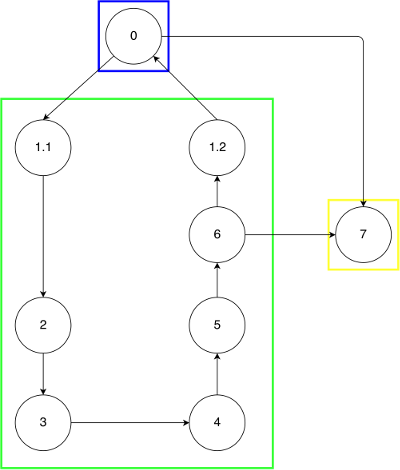
\includegraphics[width=0.3\textwidth]{images/einlagern.png}
    \caption{Einlagern}
    \label{fig:in}
  \end{center}
\end{figure}
%
\begin{figure}[H]
  \begin{center}
    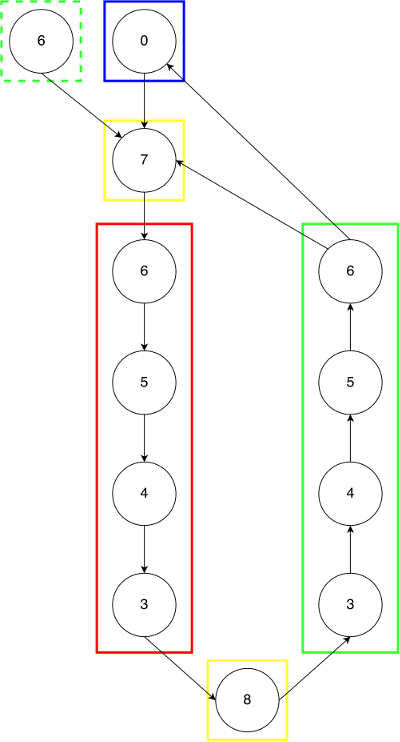
\includegraphics[width=0.3\textwidth]{images/umlagern.png}
    \caption{Umlagern}
    \label{fig:move}
  \end{center}
\end{figure}
%
\begin{figure}[H]
  \begin{center}
    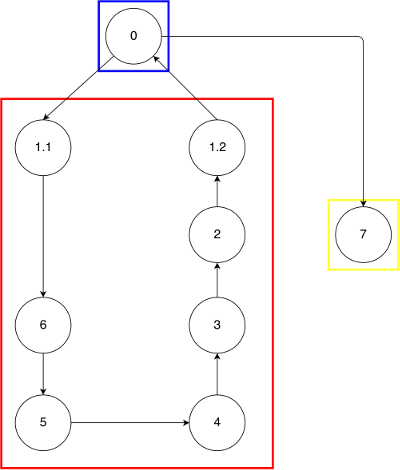
\includegraphics[width=0.3\textwidth]{images/auslagern.png}
    \caption{Auslagern}
    \label{fig:out}
  \end{center}
\end{figure}
%

\subsection{Zustände}

\subsubsection{Global}
\begin{enumerate}
  \item Get next free Gap
  \item Select Gap (first to be free?)
  \item .1 Assign Item to Bin
  \item .2 Send Item to Gap
  \item .3 Set RBG to 0.0
  \item Load Item to RBG
  \item Store Item in Bin
\end{enumerate}
%
\subsubsection{Gassen}

\paragraph{RBG Einlagern}

\begin{table}[H]
  \caption{Einlagerung}
  \label{tab:ins}

  \begin{center}
    \begin{tabular}{ccc}

		Eventnr.	& Koord.	& Zustand \\
		\hline
		1 &			0/0 	& empty\\
		2 &			0/0 	& loaded\\
		3 &			y/z 	& loaded\\
		4 	&		x 		& loaded\\
		5 &			x 		& empty\\
		6 &			y/z 	& empty\\
		1	&		0/0		& empty\\
		7 &					& sleep\\
    \end{tabular}
  \end{center}
\end{table}	
\paragraph{RBG Auslagern}

\begin{table}[H]
  \caption{Auslagerung}
  \label{tab:outs}

  \begin{center}
    \begin{tabular}{ccc}
		Eventnr.&	Koord.&	Zustand\\
		\hline
		1 &			0/0 	&empty\\
		6 &			y/z 	&empty\\
		5 &			x 		&empty\\
		4 &			x 		&loaded\\
		3 &			y/z 	&loaded\\
		2 &			0/0 	&loaded\\
		1	&		0/0		&empty\\
		7 &					&sleep \\
    \end{tabular}
  \end{center}
\end{table}	
%
\subsection{Bewegungen}



%
\subsection{Steuer-Daten}


\subsection{Architektur}
Die Unterteilung der Anwendung erfolgte in einen Teil für die Modellierung, Simulation und die Visualisierung.  





%EOF
